% Options for packages loaded elsewhere
\PassOptionsToPackage{unicode}{hyperref}
\PassOptionsToPackage{hyphens}{url}
%
\documentclass[
]{article}
\usepackage{amsmath,amssymb}
\usepackage{lmodern}
\usepackage{iftex}
\ifPDFTeX
  \usepackage[T1]{fontenc}
  \usepackage[utf8]{inputenc}
  \usepackage{textcomp} % provide euro and other symbols
\else % if luatex or xetex
  \usepackage{unicode-math}
  \defaultfontfeatures{Scale=MatchLowercase}
  \defaultfontfeatures[\rmfamily]{Ligatures=TeX,Scale=1}
\fi
% Use upquote if available, for straight quotes in verbatim environments
\IfFileExists{upquote.sty}{\usepackage{upquote}}{}
\IfFileExists{microtype.sty}{% use microtype if available
  \usepackage[]{microtype}
  \UseMicrotypeSet[protrusion]{basicmath} % disable protrusion for tt fonts
}{}
\makeatletter
\@ifundefined{KOMAClassName}{% if non-KOMA class
  \IfFileExists{parskip.sty}{%
    \usepackage{parskip}
  }{% else
    \setlength{\parindent}{0pt}
    \setlength{\parskip}{6pt plus 2pt minus 1pt}}
}{% if KOMA class
  \KOMAoptions{parskip=half}}
\makeatother
\usepackage{xcolor}
\usepackage[margin=1in]{geometry}
\usepackage{color}
\usepackage{fancyvrb}
\newcommand{\VerbBar}{|}
\newcommand{\VERB}{\Verb[commandchars=\\\{\}]}
\DefineVerbatimEnvironment{Highlighting}{Verbatim}{commandchars=\\\{\}}
% Add ',fontsize=\small' for more characters per line
\usepackage{framed}
\definecolor{shadecolor}{RGB}{248,248,248}
\newenvironment{Shaded}{\begin{snugshade}}{\end{snugshade}}
\newcommand{\AlertTok}[1]{\textcolor[rgb]{0.94,0.16,0.16}{#1}}
\newcommand{\AnnotationTok}[1]{\textcolor[rgb]{0.56,0.35,0.01}{\textbf{\textit{#1}}}}
\newcommand{\AttributeTok}[1]{\textcolor[rgb]{0.77,0.63,0.00}{#1}}
\newcommand{\BaseNTok}[1]{\textcolor[rgb]{0.00,0.00,0.81}{#1}}
\newcommand{\BuiltInTok}[1]{#1}
\newcommand{\CharTok}[1]{\textcolor[rgb]{0.31,0.60,0.02}{#1}}
\newcommand{\CommentTok}[1]{\textcolor[rgb]{0.56,0.35,0.01}{\textit{#1}}}
\newcommand{\CommentVarTok}[1]{\textcolor[rgb]{0.56,0.35,0.01}{\textbf{\textit{#1}}}}
\newcommand{\ConstantTok}[1]{\textcolor[rgb]{0.00,0.00,0.00}{#1}}
\newcommand{\ControlFlowTok}[1]{\textcolor[rgb]{0.13,0.29,0.53}{\textbf{#1}}}
\newcommand{\DataTypeTok}[1]{\textcolor[rgb]{0.13,0.29,0.53}{#1}}
\newcommand{\DecValTok}[1]{\textcolor[rgb]{0.00,0.00,0.81}{#1}}
\newcommand{\DocumentationTok}[1]{\textcolor[rgb]{0.56,0.35,0.01}{\textbf{\textit{#1}}}}
\newcommand{\ErrorTok}[1]{\textcolor[rgb]{0.64,0.00,0.00}{\textbf{#1}}}
\newcommand{\ExtensionTok}[1]{#1}
\newcommand{\FloatTok}[1]{\textcolor[rgb]{0.00,0.00,0.81}{#1}}
\newcommand{\FunctionTok}[1]{\textcolor[rgb]{0.00,0.00,0.00}{#1}}
\newcommand{\ImportTok}[1]{#1}
\newcommand{\InformationTok}[1]{\textcolor[rgb]{0.56,0.35,0.01}{\textbf{\textit{#1}}}}
\newcommand{\KeywordTok}[1]{\textcolor[rgb]{0.13,0.29,0.53}{\textbf{#1}}}
\newcommand{\NormalTok}[1]{#1}
\newcommand{\OperatorTok}[1]{\textcolor[rgb]{0.81,0.36,0.00}{\textbf{#1}}}
\newcommand{\OtherTok}[1]{\textcolor[rgb]{0.56,0.35,0.01}{#1}}
\newcommand{\PreprocessorTok}[1]{\textcolor[rgb]{0.56,0.35,0.01}{\textit{#1}}}
\newcommand{\RegionMarkerTok}[1]{#1}
\newcommand{\SpecialCharTok}[1]{\textcolor[rgb]{0.00,0.00,0.00}{#1}}
\newcommand{\SpecialStringTok}[1]{\textcolor[rgb]{0.31,0.60,0.02}{#1}}
\newcommand{\StringTok}[1]{\textcolor[rgb]{0.31,0.60,0.02}{#1}}
\newcommand{\VariableTok}[1]{\textcolor[rgb]{0.00,0.00,0.00}{#1}}
\newcommand{\VerbatimStringTok}[1]{\textcolor[rgb]{0.31,0.60,0.02}{#1}}
\newcommand{\WarningTok}[1]{\textcolor[rgb]{0.56,0.35,0.01}{\textbf{\textit{#1}}}}
\usepackage{longtable,booktabs,array}
\usepackage{calc} % for calculating minipage widths
% Correct order of tables after \paragraph or \subparagraph
\usepackage{etoolbox}
\makeatletter
\patchcmd\longtable{\par}{\if@noskipsec\mbox{}\fi\par}{}{}
\makeatother
% Allow footnotes in longtable head/foot
\IfFileExists{footnotehyper.sty}{\usepackage{footnotehyper}}{\usepackage{footnote}}
\makesavenoteenv{longtable}
\usepackage{graphicx}
\makeatletter
\def\maxwidth{\ifdim\Gin@nat@width>\linewidth\linewidth\else\Gin@nat@width\fi}
\def\maxheight{\ifdim\Gin@nat@height>\textheight\textheight\else\Gin@nat@height\fi}
\makeatother
% Scale images if necessary, so that they will not overflow the page
% margins by default, and it is still possible to overwrite the defaults
% using explicit options in \includegraphics[width, height, ...]{}
\setkeys{Gin}{width=\maxwidth,height=\maxheight,keepaspectratio}
% Set default figure placement to htbp
\makeatletter
\def\fps@figure{htbp}
\makeatother
\setlength{\emergencystretch}{3em} % prevent overfull lines
\providecommand{\tightlist}{%
  \setlength{\itemsep}{0pt}\setlength{\parskip}{0pt}}
\setcounter{secnumdepth}{-\maxdimen} % remove section numbering
\ifLuaTeX
  \usepackage{selnolig}  % disable illegal ligatures
\fi
\IfFileExists{bookmark.sty}{\usepackage{bookmark}}{\usepackage{hyperref}}
\IfFileExists{xurl.sty}{\usepackage{xurl}}{} % add URL line breaks if available
\urlstyle{same} % disable monospaced font for URLs
\hypersetup{
  pdftitle={The P600 effect when singular gendered antecedents are co-indexed with (a) himself or herself (b) themselves},
  pdfauthor={Joanna Morris},
  hidelinks,
  pdfcreator={LaTeX via pandoc}}

\title{The P600 effect when singular gendered antecedents are co-indexed
with (a) \emph{himself} or \emph{herself} (b) \emph{themselves}}
\author{Joanna Morris}
\date{2023-02-13}

\begin{document}
\maketitle

\hypertarget{define-functions-set-parameters-and-load}{%
\subsection{Define functions, set parameters and
load}\label{define-functions-set-parameters-and-load}}

Define standard error of mean function

\begin{Shaded}
\begin{Highlighting}[]
\NormalTok{sem }\OtherTok{\textless{}{-}} \ControlFlowTok{function}\NormalTok{(x) }\FunctionTok{sd}\NormalTok{(x)}\SpecialCharTok{/}\FunctionTok{sqrt}\NormalTok{(}\FunctionTok{length}\NormalTok{(x))}
\end{Highlighting}
\end{Shaded}

Before we begin, let's set some general parameters for \texttt{ggplot2}.
We will set a general theme using the \texttt{theme\_set()} function. We
will use the `classic' theme which gives us clean white background
rather than the default grey with white grid lines. And we will position
the legend at the top of the graph rather than at the right side which
is the default.

Then we re-order factor levels for \emph{Referentiality}

\begin{verbatim}
## [1] "Referential"    "NonReferential"
\end{verbatim}

\begin{verbatim}
## [1] "Referential"    "NonReferential"
\end{verbatim}

\hypertarget{analysis-1-the-p600-effect-when-antecedents-are-co-indexed-with-himself-or-herself}{%
\subsection{\texorpdfstring{Analysis 1: The P600 effect when antecedents
are co-indexed with \emph{himself} or
\emph{herself}}{Analysis 1: The P600 effect when antecedents are co-indexed with himself or herself}}\label{analysis-1-the-p600-effect-when-antecedents-are-co-indexed-with-himself-or-herself}}

\begin{Shaded}
\begin{Highlighting}[]
\FunctionTok{ezANOVA}\NormalTok{(}\AttributeTok{data =}\NormalTok{ prost\_2022\_singular}
\NormalTok{              , }\AttributeTok{dv =}\NormalTok{ diff\_score}
\NormalTok{              , }\AttributeTok{wid =}\NormalTok{ SubjID}
\NormalTok{              , }\AttributeTok{within =}\NormalTok{ .(Referentiality, Gender\_Status)}
\NormalTok{              , }\AttributeTok{between =}\NormalTok{ Group}
\NormalTok{              , }\AttributeTok{type =} \DecValTok{3}
\NormalTok{              , }\AttributeTok{return\_aov =}\NormalTok{ F}
\NormalTok{              )}
\end{Highlighting}
\end{Shaded}

\begin{verbatim}
## $ANOVA
##                               Effect DFn DFd          F            p p<.05
## 2                              Group   1  36  2.6476957 1.124226e-01      
## 3                     Referentiality   1  36 24.2580517 1.887572e-05     *
## 5                      Gender_Status   1  36  2.1030534 1.556627e-01      
## 4               Group:Referentiality   1  36  0.2741019 6.038016e-01      
## 6                Group:Gender_Status   1  36  0.2164015 6.445974e-01      
## 7       Referentiality:Gender_Status   1  36  5.1551114 2.926166e-02     *
## 8 Group:Referentiality:Gender_Status   1  36  2.0276871 1.630661e-01      
##           ges
## 2 0.016408837
## 3 0.165071951
## 5 0.016550569
## 4 0.002229006
## 6 0.001728699
## 7 0.026715413
## 8 0.010681228
\end{verbatim}

\hypertarget{condition-means-for-analysis-1}{%
\subsubsection{Condition Means for Analysis
1}\label{condition-means-for-analysis-1}}

The P600 effect when antecedents are co-indexed with \emph{himself} or
\emph{herself}.

Significant Effects: \textbf{Referentiality; Group x Referentiality x
Gender Status}

\begin{longtable}[]{@{}lrrrrr@{}}
\toprule()
Referentiality & Mean & SE & SD & Max & Min \\
\midrule()
\endhead
Referential & -0.34 & 0.16 & 1.42 & 4.15 & -4.41 \\
NonReferential & 1.03 & 0.20 & 1.78 & 6.52 & -3.33 \\
\bottomrule()
\end{longtable}

\begin{longtable}[]{@{}lrrrrr@{}}
\toprule()
Gender\_Status & Mean & SE & SD & Max & Min \\
\midrule()
\endhead
Gendered & 0.54 & 0.23 & 1.97 & 6.52 & -4.41 \\
NonGendered & 0.15 & 0.17 & 1.47 & 4.02 & -3.33 \\
\bottomrule()
\end{longtable}

\begin{longtable}[]{@{}lrrrrr@{}}
\toprule()
Group & Mean & SE & SD & Max & Min \\
\midrule()
\endhead
Binary & 0.16 & 0.2 & 1.75 & 5.10 & -4.41 \\
NonBinary & 0.56 & 0.2 & 1.73 & 6.52 & -2.63 \\
\bottomrule()
\end{longtable}

\begin{longtable}[]{@{}
  >{\raggedright\arraybackslash}p{(\columnwidth - 14\tabcolsep) * \real{0.2273}}
  >{\raggedright\arraybackslash}p{(\columnwidth - 14\tabcolsep) * \real{0.2121}}
  >{\raggedright\arraybackslash}p{(\columnwidth - 14\tabcolsep) * \real{0.1515}}
  >{\raggedleft\arraybackslash}p{(\columnwidth - 14\tabcolsep) * \real{0.0909}}
  >{\raggedleft\arraybackslash}p{(\columnwidth - 14\tabcolsep) * \real{0.0758}}
  >{\raggedleft\arraybackslash}p{(\columnwidth - 14\tabcolsep) * \real{0.0758}}
  >{\raggedleft\arraybackslash}p{(\columnwidth - 14\tabcolsep) * \real{0.0758}}
  >{\raggedleft\arraybackslash}p{(\columnwidth - 14\tabcolsep) * \real{0.0909}}@{}}
\toprule()
\begin{minipage}[b]{\linewidth}\raggedright
Referentiality
\end{minipage} & \begin{minipage}[b]{\linewidth}\raggedright
Gender\_Status
\end{minipage} & \begin{minipage}[b]{\linewidth}\raggedright
Group
\end{minipage} & \begin{minipage}[b]{\linewidth}\raggedleft
Mean
\end{minipage} & \begin{minipage}[b]{\linewidth}\raggedleft
SE
\end{minipage} & \begin{minipage}[b]{\linewidth}\raggedleft
SD
\end{minipage} & \begin{minipage}[b]{\linewidth}\raggedleft
Max
\end{minipage} & \begin{minipage}[b]{\linewidth}\raggedleft
Min
\end{minipage} \\
\midrule()
\endhead
Referential & Gendered & Binary & -0.74 & 0.41 & 1.85 & 4.15 & -4.41 \\
Referential & Gendered & NonBinary & -0.04 & 0.31 & 1.31 & 2.48 &
-2.04 \\
Referential & NonGendered & Binary & -0.18 & 0.27 & 1.19 & 2.54 &
-2.15 \\
Referential & NonGendered & NonBinary & -0.37 & 0.28 & 1.21 & 1.73 &
-2.50 \\
NonReferential & Gendered & Binary & 1.32 & 0.40 & 1.77 & 5.10 &
-1.66 \\
NonReferential & Gendered & NonBinary & 1.67 & 0.46 & 1.94 & 6.52 &
-0.59 \\
NonReferential & NonGendered & Binary & 0.22 & 0.34 & 1.54 & 4.02 &
-3.33 \\
NonReferential & NonGendered & NonBinary & 0.95 & 0.39 & 1.66 & 3.40 &
-2.63 \\
\bottomrule()
\end{longtable}

\hypertarget{post-hoc-tests-for-analysis-1-group-x-gender-status-x-referentiality}{%
\subsubsection{Post-hoc tests for Analysis 1: Group x Gender Status x
Referentiality}\label{post-hoc-tests-for-analysis-1-group-x-gender-status-x-referentiality}}

The following chunk runs post-hoc tests for the 3-way
\textbf{\emph{``Group x Gender Status x Referentiality''}} Interaction

``Some woman\ldots himself'' vs.~``Mary\ldots himself''

\begin{longtable}[]{@{}
  >{\centering\arraybackslash}p{(\columnwidth - 8\tabcolsep) * \real{0.2073}}
  >{\centering\arraybackslash}p{(\columnwidth - 8\tabcolsep) * \real{0.0610}}
  >{\centering\arraybackslash}p{(\columnwidth - 8\tabcolsep) * \real{0.2073}}
  >{\centering\arraybackslash}p{(\columnwidth - 8\tabcolsep) * \real{0.3049}}
  >{\centering\arraybackslash}p{(\columnwidth - 8\tabcolsep) * \real{0.2195}}@{}}
\caption{Paired t-test: \texttt{diff\_score} by
\texttt{Referentiality}}\tabularnewline
\toprule()
\begin{minipage}[b]{\linewidth}\centering
Test statistic
\end{minipage} & \begin{minipage}[b]{\linewidth}\centering
df
\end{minipage} & \begin{minipage}[b]{\linewidth}\centering
P value
\end{minipage} & \begin{minipage}[b]{\linewidth}\centering
Alternative hypothesis
\end{minipage} & \begin{minipage}[b]{\linewidth}\centering
mean difference
\end{minipage} \\
\midrule()
\endfirsthead
\toprule()
\begin{minipage}[b]{\linewidth}\centering
Test statistic
\end{minipage} & \begin{minipage}[b]{\linewidth}\centering
df
\end{minipage} & \begin{minipage}[b]{\linewidth}\centering
P value
\end{minipage} & \begin{minipage}[b]{\linewidth}\centering
Alternative hypothesis
\end{minipage} & \begin{minipage}[b]{\linewidth}\centering
mean difference
\end{minipage} \\
\midrule()
\endhead
-4.833 & 37 & 2.36e-05 * * * & two.sided & -1.893 \\
\bottomrule()
\end{longtable}

``Someone\ldots himself'' vs.~``The participant\ldots himself''

\begin{longtable}[]{@{}
  >{\centering\arraybackslash}p{(\columnwidth - 8\tabcolsep) * \real{0.2208}}
  >{\centering\arraybackslash}p{(\columnwidth - 8\tabcolsep) * \real{0.0649}}
  >{\centering\arraybackslash}p{(\columnwidth - 8\tabcolsep) * \real{0.1558}}
  >{\centering\arraybackslash}p{(\columnwidth - 8\tabcolsep) * \real{0.3247}}
  >{\centering\arraybackslash}p{(\columnwidth - 8\tabcolsep) * \real{0.2338}}@{}}
\caption{Paired t-test: \texttt{diff\_score} by
\texttt{Referentiality}}\tabularnewline
\toprule()
\begin{minipage}[b]{\linewidth}\centering
Test statistic
\end{minipage} & \begin{minipage}[b]{\linewidth}\centering
df
\end{minipage} & \begin{minipage}[b]{\linewidth}\centering
P value
\end{minipage} & \begin{minipage}[b]{\linewidth}\centering
Alternative hypothesis
\end{minipage} & \begin{minipage}[b]{\linewidth}\centering
mean difference
\end{minipage} \\
\midrule()
\endfirsthead
\toprule()
\begin{minipage}[b]{\linewidth}\centering
Test statistic
\end{minipage} & \begin{minipage}[b]{\linewidth}\centering
df
\end{minipage} & \begin{minipage}[b]{\linewidth}\centering
P value
\end{minipage} & \begin{minipage}[b]{\linewidth}\centering
Alternative hypothesis
\end{minipage} & \begin{minipage}[b]{\linewidth}\centering
mean difference
\end{minipage} \\
\midrule()
\endhead
-2.614 & 37 & 0.01286 * & two.sided & -0.8365 \\
\bottomrule()
\end{longtable}

``The participant\ldots himself'' vs.~``Mary\ldots himself''

\begin{longtable}[]{@{}
  >{\centering\arraybackslash}p{(\columnwidth - 8\tabcolsep) * \real{0.2267}}
  >{\centering\arraybackslash}p{(\columnwidth - 8\tabcolsep) * \real{0.0667}}
  >{\centering\arraybackslash}p{(\columnwidth - 8\tabcolsep) * \real{0.1333}}
  >{\centering\arraybackslash}p{(\columnwidth - 8\tabcolsep) * \real{0.3333}}
  >{\centering\arraybackslash}p{(\columnwidth - 8\tabcolsep) * \real{0.2400}}@{}}
\caption{Paired t-test: \texttt{diff\_score} by
\texttt{Gender\_Status}}\tabularnewline
\toprule()
\begin{minipage}[b]{\linewidth}\centering
Test statistic
\end{minipage} & \begin{minipage}[b]{\linewidth}\centering
df
\end{minipage} & \begin{minipage}[b]{\linewidth}\centering
P value
\end{minipage} & \begin{minipage}[b]{\linewidth}\centering
Alternative hypothesis
\end{minipage} & \begin{minipage}[b]{\linewidth}\centering
mean difference
\end{minipage} \\
\midrule()
\endfirsthead
\toprule()
\begin{minipage}[b]{\linewidth}\centering
Test statistic
\end{minipage} & \begin{minipage}[b]{\linewidth}\centering
df
\end{minipage} & \begin{minipage}[b]{\linewidth}\centering
P value
\end{minipage} & \begin{minipage}[b]{\linewidth}\centering
Alternative hypothesis
\end{minipage} & \begin{minipage}[b]{\linewidth}\centering
mean difference
\end{minipage} \\
\midrule()
\endhead
-0.3661 & 37 & 0.7164 & two.sided & -0.1346 \\
\bottomrule()
\end{longtable}

``Someone\ldots himself'' vs.~``Some woman\ldots himself''

\begin{longtable}[]{@{}
  >{\centering\arraybackslash}p{(\columnwidth - 8\tabcolsep) * \real{0.2208}}
  >{\centering\arraybackslash}p{(\columnwidth - 8\tabcolsep) * \real{0.0649}}
  >{\centering\arraybackslash}p{(\columnwidth - 8\tabcolsep) * \real{0.1558}}
  >{\centering\arraybackslash}p{(\columnwidth - 8\tabcolsep) * \real{0.3247}}
  >{\centering\arraybackslash}p{(\columnwidth - 8\tabcolsep) * \real{0.2338}}@{}}
\caption{Paired t-test: \texttt{diff\_score} by
\texttt{Gender\_Status}}\tabularnewline
\toprule()
\begin{minipage}[b]{\linewidth}\centering
Test statistic
\end{minipage} & \begin{minipage}[b]{\linewidth}\centering
df
\end{minipage} & \begin{minipage}[b]{\linewidth}\centering
P value
\end{minipage} & \begin{minipage}[b]{\linewidth}\centering
Alternative hypothesis
\end{minipage} & \begin{minipage}[b]{\linewidth}\centering
mean difference
\end{minipage} \\
\midrule()
\endfirsthead
\toprule()
\begin{minipage}[b]{\linewidth}\centering
Test statistic
\end{minipage} & \begin{minipage}[b]{\linewidth}\centering
df
\end{minipage} & \begin{minipage}[b]{\linewidth}\centering
P value
\end{minipage} & \begin{minipage}[b]{\linewidth}\centering
Alternative hypothesis
\end{minipage} & \begin{minipage}[b]{\linewidth}\centering
mean difference
\end{minipage} \\
\midrule()
\endhead
2.688 & 37 & 0.01071 * & two.sided & 0.9219 \\
\bottomrule()
\end{longtable}

\hypertarget{interaction-plots-gender-status-x-referentiality-himself}{%
\subparagraph{\texorpdfstring{Interaction Plots: Gender Status x
Referentiality
\emph{himself}}{Interaction Plots: Gender Status x Referentiality himself}}\label{interaction-plots-gender-status-x-referentiality-himself}}

~

\includegraphics{prost_2022_p600_b_files/figure-latex/unnamed-chunk-10-1.pdf}

Interaction broken down by Group \emph{Binary} vs \emph{Non-Binary}

\includegraphics{prost_2022_p600_b_files/figure-latex/unnamed-chunk-11-1.pdf}

\includegraphics{prost_2022_p600_b_files/figure-latex/unnamed-chunk-12-1.pdf}

\hypertarget{analysis-2-the-p600-effect-when-antecedents-are-co-indexed-with-themselves}{%
\subsection{\texorpdfstring{Analysis 2: The P600 effect when antecedents
are co-indexed with
\emph{themselves}}{Analysis 2: The P600 effect when antecedents are co-indexed with themselves}}\label{analysis-2-the-p600-effect-when-antecedents-are-co-indexed-with-themselves}}

\begin{Shaded}
\begin{Highlighting}[]
\FunctionTok{ezANOVA}\NormalTok{(}\AttributeTok{data =}\NormalTok{ prost\_2022\_plural}
\NormalTok{              , }\AttributeTok{dv =}\NormalTok{ diff\_score}
\NormalTok{              , }\AttributeTok{wid =}\NormalTok{ SubjID}
\NormalTok{              , }\AttributeTok{within =}\NormalTok{ .(Referentiality, Gender\_Status)}
\NormalTok{              , }\AttributeTok{between =}\NormalTok{ Group}
\NormalTok{              , }\AttributeTok{type =} \DecValTok{3}
\NormalTok{              , }\AttributeTok{return\_aov =}\NormalTok{ F}
\NormalTok{              )}
\end{Highlighting}
\end{Shaded}

\begin{verbatim}
## $ANOVA
##                               Effect DFn DFd            F          p p<.05
## 2                              Group   1  36 0.0053411590 0.94214444      
## 3                     Referentiality   1  36 5.2198710296 0.02832801     *
## 5                      Gender_Status   1  36 0.5605028582 0.45892150      
## 4               Group:Referentiality   1  36 0.0000511147 0.99433508      
## 6                Group:Gender_Status   1  36 0.0456034989 0.83210302      
## 7       Referentiality:Gender_Status   1  36 5.0012917068 0.03161659     *
## 8 Group:Referentiality:Gender_Status   1  36 1.1780250752 0.28497330      
##            ges
## 2 3.760513e-05
## 3 2.392545e-02
## 5 3.402687e-03
## 4 2.400287e-07
## 6 2.777167e-04
## 7 4.740160e-02
## 8 1.158497e-02
\end{verbatim}

\hypertarget{interaction-plots-gender-status-by-referentiality-themselves}{%
\paragraph{\texorpdfstring{Interaction Plots: Gender Status by
Referentiality
\emph{themselves}}{Interaction Plots: Gender Status by Referentiality themselves}}\label{interaction-plots-gender-status-by-referentiality-themselves}}

~

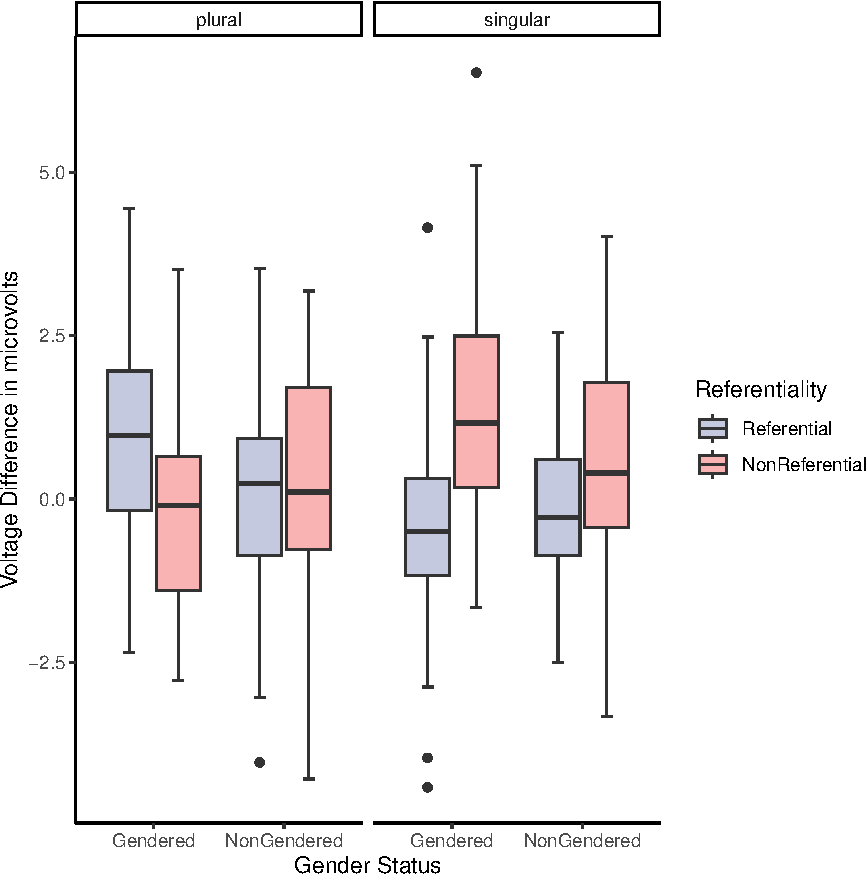
\includegraphics{prost_2022_p600_b_files/figure-latex/unnamed-chunk-14-1.pdf}

Interaction broken down by Group \emph{Binary} vs \emph{Non-Binary}

\includegraphics{prost_2022_p600_b_files/figure-latex/unnamed-chunk-15-1.pdf}

~

\includegraphics{prost_2022_p600_b_files/figure-latex/unnamed-chunk-16-1.pdf}

\end{document}
